\documentclass{article}
\usepackage[utf8]{inputenc}
\usepackage{tikz}

\title{TikZ Test}
\author{Jesse He}
\date{16 July 2019}

\begin{document}

\maketitle

This is a line.
\begin{tikzpicture}
    \draw (0,0) -- (2,0);
\end{tikzpicture}\newline

This is a square.
\begin{tikzpicture}
    \draw (0,0)--(2,0)--(2,2)--(0,2)--cycle;
\end{tikzpicture}\newline

This is a parabola.
\begin{tikzpicture}
    \draw (0,0) parabola (-2,2) (0,0) parabola (2,2);
\end{tikzpicture}\newline

This is a curved line.
\begin{tikzpicture}
    \draw (0,0) .. controls (0,2) and (2,0) .. (2,2);
\end{tikzpicture}\newline

This is a circle, an ellipse, and an arc.
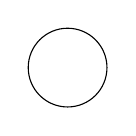
\begin{tikzpicture}
    \draw (0,0) circle (.5cm);
\end{tikzpicture}
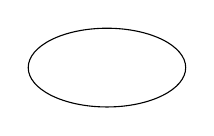
\begin{tikzpicture}
    \draw (0,0) ellipse (1cm and .5cm);
\end{tikzpicture}
\begin{tikzpicture}
    \draw (0,0) arc (0:90:.5cm);
\end{tikzpicture}\newline

This is a graph of $y=x^2$.
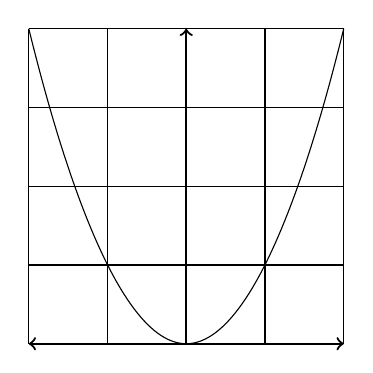
\begin{tikzpicture}
    \draw[step=1cm,thin] (-2,0) grid (2,4);
    \draw[thick,->] (0,0)--(0,4);
    \draw[thick,<->] (-2,0)--(2,0);
    \draw (0,0) parabola (-2,4) (0,0) parabola (2,4);
\end{tikzpicture}\newline

This is a Riemann sum for $\int_0^2 x^2 dx$.
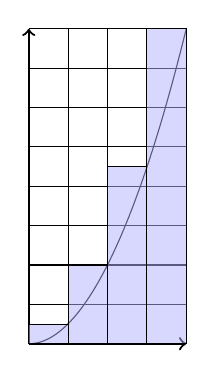
\begin{tikzpicture}
    \draw[step=.5cm,thin] (0,0) grid (2,4);
    \draw[thick,->] (0,0)--(0,4);
    \draw[thick,->] (0,0)--(2,0);
    \draw (0,0) parabola (2,4);
    \filldraw[fill=blue!30!white,fill opacity=0.5,draw=black] (0,0) rectangle (.5,.25);
    \filldraw[fill=blue!30!white,fill opacity=0.5,draw=black] (.5,0) rectangle (1,1);
    \filldraw[fill=blue!30!white,fill opacity=0.5,draw=black] (1,0) rectangle (1.5,2.25);
    \filldraw[fill=blue!30!white,fill opacity=0.5,draw=black] (1.5,0) rectangle (2,4);
\end{tikzpicture}\newline

\end{document}